\documentclass[aspectratio=1610]{beamer}
\usetheme{KTH}
\usepackage[utf8]{inputenc}
\usepackage[T1]{fontenc}
\usepackage[format=hang]{caption}
\usepackage{subcaption}
\captionsetup{font=normalsize,labelfont={bf,sf}}
\captionsetup[sub]{font={small}, textfont={normalfont}, labelfont={bf,sf}}
\usepackage{pgfplots}
\pgfplotsset{compat=1.14}
\usepackage[export]{adjustbox}

\usepackage{tikz}
\usepackage{tikzpeople}
\usetikzlibrary{shapes,arrows.meta,positioning,automata,matrix,shapes.symbols,shapes.misc}

\usepackage{libertine}
\usepackage{sourcecodepro}
\usepackage{fontawesome}

\usepackage{todonotes}
\usepackage{wrapfig}
\usepackage[binary-units]{siunitx}
\sisetup{
    detect-all,
    detect-inline-family=math,
    detect-inline-weight=math,
    detect-display-math=true
}
\DeclareSIUnit{\belmilliwatt}{Bm}
\DeclareSIUnit{\dBm}{\deci\belmilliwatt}

%\usepackage[hidelinks]{hyperref}

\newcommand{\emailref}[1]{\href{mailto:#1}{\texttt{#1}}}
\newcommand{\telref}[1]{\href{tel:#1}{\texttt{#1}}}
\newcommand{\urlref}[1]{\href{#1}{\texttt{#1}}}

\usepackage[style=ieee,
    backend=bibtex,
    sorting=none,
    sortcites,
    maxbibnames=1,
    minbibnames=1,
    maxcitenames=2,
    mincitenames=1]{biblatex}
\AtBeginBibliography{\footnotesize}
\addbibresource{bibliography.bib}


\newcommand{\icontag}[2]{
    #1~#2\\
}

%% TOC before each section

\AtBeginSection[]
{
    \begin{frame}<beamer>
        \frametitle{Outline}
        \setcounter{tocdepth}{2}%
        \tableofcontents[currentsection,hideothersubsections]
    \end{frame}
}

\AtEndDocument%
{
    \startpage
    \begin{frame}
        \begin{center}
            \begin{Large}
                \textbf{Thank you!}\\
            \end{Large}
            \vspace{.1\textheight}
            \begin{footnotesize}
                \icontag{\faAt}{\href{mailto:molguin@kth.se}{\texttt{molguin@kth.se}}}
                \icontag{\faTwitter}{\href{https://twitter.com/molguin92}{\texttt{@molguin92}}}
                \icontag{\faGithub}{\href{https://github.com/molguin92}{\texttt{molguin92}}}
            \end{footnotesize}
        \end{center}

    \end{frame}
    \normalpage
}

\newcommand{\kthaffil}{\textsuperscript{\textdagger}}
\newcommand{\cmuaffil}{\textsuperscript{\textdaggerdbl}}

\begin{document}
\startpage
%%%%%%%%%%%%%%%%%%%%%%%%%%%%%%%%%%%%%%%%%%%%%%%%%%%%%%%%%%%%
\begin{frame}{}
    \begin{center}
        \begin{LARGE}
            \textbf{EdgeDroid}\\
        \end{LARGE}
        \emph{An Experimental Approach to Benchmarking Human-in-the-Loop Applications}\\
        \vspace{0.02\textheight}
        {\footnotesize \underline{M. Olguín Muñoz}\kthaffil, J. Wang\cmuaffil, M. Satyanarayanan\cmuaffil and J. Gross\kthaffil\\
            \vspace{0.02\textheight}
            \kthaffil~KTH Royal Institute of Technology\\
            \cmuaffil~Carnegie Mellon University\\}
    \end{center}

    \vspace{0.04\textheight}

    \begin{tiny}
        \raggedleft%
        \emph{HotMobile'19 Session 5: February 28\textsuperscript{th} 2019, Santa Cruz, CA}\\
    \end{tiny}
\end{frame}

\normalpage%
{
    % within group to not have an outline for the first section
    \AtBeginSection[]{}
    \section{Introduction}
}

\begin{frame}{Introduction}
    \note{Introduce human-in-the-loop and cognitive assistance}

    \begin{center}
        \begin{tikzpicture}
            \node [inner sep=0mm] (ironman) {\includegraphics[width=.8\linewidth]{img/ar_ironman.png}};

            \path (ironman.east) -- coordinate[midway] (anchor) (ironman.south east);

            \node [inner sep=0mm] (pokemongo) at (anchor)  {\includegraphics[width=.5\linewidth]{img/ar_pokemongo.jpg}};
        \end{tikzpicture}
    \end{center}
    
\end{frame}

\begin{frame}{Human-in-the-Loop Applications}
    \begin{columns}[onlytextwidth]
        \begin{column}{.335\linewidth}%filler
        \end{column}%
        \begin{column}{.1\linewidth}
            \centering%
            \includegraphics[width=\linewidth]{img/sound_wave.png}
        \end{column}%
        \begin{column}{.01\linewidth}
        \end{column}%
        \begin{column}{.1\linewidth}
            \centering%
            \includegraphics[width=\linewidth]{img/film.png}
        \end{column}%
        \begin{column}{.01\linewidth}
        \end{column}%
        \begin{column}{.1\linewidth}
            \centering%
            \includegraphics[width=\linewidth]{img/accel.png}
        \end{column}%
        \begin{column}{.335\linewidth}%filler
        \end{column}%
    \end{columns}%
    \begin{columns}[onlytextwidth]
        \begin{column}{.25\linewidth}
            \centering%
            \includegraphics[width=\linewidth]{img/glass_wearable.jpeg}\\
        \end{column}
        \begin{column}{.5\linewidth}
            \centering
            \begin{tikzpicture}[align=center,
    node distance=0.7cm and 0.7cm,
    every initial by arrow/.style={draw=none, minimum size=0em},
    %node styles:
    block_center/.style ={rectangle, draw=black, thick, fill=white,
            text width=8em, text centered, minimum height=4em},
    block_left/.style ={rectangle, draw=black, thick, fill=white,
            text width=16em, text ragged, minimum height=4em, inner sep=6pt},
    block_noborder/.style ={rectangle, draw=none, thick, fill=none,
            text width=18em, text centered, minimum height=1em},
    block_assign/.style ={rectangle, draw=black, thick, fill=white,
            text width=18em, text ragged, minimum height=3em, inner sep=6pt},
    block_lost/.style ={rectangle, draw=black, thick, fill=white,
            text width=16em, text ragged, minimum height=3em, inner sep=6pt},
    block_rounded/.style ={rectangle, draw=black, thick, fill=white,
            text width=8em, text centered, rounded corners=.55cm, minimum height=4em},
    line/.style ={draw, very thick, line cap=round, -{Latex[length=2.5mm]}, shorten >=0pt}
    ]

    \matrix [column sep=20mm,row sep=3mm] (mtx) {
        \node[inner sep=0pt] (user) {\includegraphics[height=.2\textheight]{img/google-glass.png}};
         & \node [inner sep=0pt] (server) {\includegraphics[height=.2\textheight]{img/server.png}}; \\
    };


    \path[draw, line]
    (user) edge [out=45, in=135] node[above] {Sensory Input} (server)
    (server) edge [out=225, in=315] node[below] {Human-parseable\\Feedback} (user);
\end{tikzpicture}%
        \end{column}%
        \begin{column}{.25\linewidth}
            \centering%
            \includegraphics[width=\linewidth]{img/NN.png}\\
        \end{column}%
    \end{columns}%
    \begin{columns}[onlytextwidth]
        \begin{column}{.335\linewidth}%filler
        \end{column}%
        \begin{column}{.1\linewidth}
            \centering%
            \includegraphics[width=\linewidth]{img/sound_wave.png}
        \end{column}%
        \begin{column}{.01\linewidth}
        \end{column}%
        \begin{column}{.1\linewidth}
            \centering%
            \includegraphics[width=\linewidth]{img/film.png}
        \end{column}%
        \begin{column}{.01\linewidth}
        \end{column}%
        \begin{column}{.1\linewidth}
            \centering%
            \includegraphics[width=\linewidth]{img/vibration.png}
        \end{column}%
        \begin{column}{.335\linewidth}%filler
        \end{column}%
    \end{columns}
\end{frame}

\begin{frame}{Scaling}
    \begin{center}
        \begin{tikzpicture}[align=center,
    node distance=0.7cm and 0.7cm,
    every initial by arrow/.style={draw=none, minimum size=0em},
    %node styles:
    block_center/.style ={rectangle, draw=black, thick, fill=white,
            text width=8em, text centered, minimum height=4em},
    block_left/.style ={rectangle, draw=black, thick, fill=white,
            text width=16em, text ragged, minimum height=4em, inner sep=6pt},
    block_noborder/.style ={rectangle, draw=none, thick, fill=none,
            text width=18em, text centered, minimum height=1em},
    block_assign/.style ={rectangle, draw=black, thick, fill=white,
            text width=18em, text ragged, minimum height=3em, inner sep=6pt},
    block_lost/.style ={rectangle, draw=black, thick, fill=white,
            text width=16em, text ragged, minimum height=3em, inner sep=6pt},
    block_rounded/.style ={rectangle, draw=black, thick, fill=white,
            text width=8em, text centered, rounded corners=.55cm, minimum height=4em},
    line/.style ={draw, very thick, line cap=round, -{Latex[length=2.5mm]}, shorten >=0pt}
    ]

    \matrix [column sep=20mm,row sep=3mm] (mtx) {
        \node[inner sep=0pt] (user) {\includegraphics[height=.2\textheight]{img/google-glass.png}};
         & \node [inner sep=0pt] (server) {\includegraphics[height=.2\textheight]{img/server.png}}; \\
    };


    \path[draw, line]
    (user) edge [out=45, in=135] node[above] {Sensory Input} (server)
    (server) edge [out=225, in=315] node[below] {Human-parseable\\Feedback} (user);
\end{tikzpicture}\\% % change to image of scaling
        \vspace{.1\textheight}%
        No solution yet?
    \end{center}
\end{frame}

\begin{frame}{Our Contributions}
    \begin{itemize}
        \itemsep2em
        \onslide<2->{\item A methodology for benchmarking human-in-the-loop applications.}
        \onslide<3->{\item EdgeDroid: A benchmarking tool-suite.}
        \onslide<4->{\item A set of experiments and measurements which show the effectiveness of the approach.}
    \end{itemize}
\end{frame}

\section{Background}
\subsection{Previous \& Related Work}
\begin{frame}{Previous \& Related Work}
    
\end{frame}


\subsection{Motivation}

\begin{frame}{Motivation}
    \begin{center}
        \only<1>{%
            \begin{tikzpicture}[align=center,
    node distance=0.7cm and 0.7cm,
    every initial by arrow/.style={draw=none, minimum size=0em},
    %node styles:
    block_center/.style ={rectangle, draw=black, thick, fill=white,
            text width=8em, text centered, minimum height=4em},
    block_left/.style ={rectangle, draw=black, thick, fill=white,
            text width=16em, text ragged, minimum height=4em, inner sep=6pt},
    block_noborder/.style ={rectangle, draw=none, thick, fill=none,
            text width=18em, text centered, minimum height=1em},
    block_assign/.style ={rectangle, draw=black, thick, fill=white,
            text width=18em, text ragged, minimum height=3em, inner sep=6pt},
    block_lost/.style ={rectangle, draw=black, thick, fill=white,
            text width=16em, text ragged, minimum height=3em, inner sep=6pt},
    block_rounded/.style ={rectangle, draw=black, thick, fill=white,
            text width=8em, text centered, rounded corners=.55cm, minimum height=4em},
    line/.style ={draw, very thick, line cap=round, -{Latex[length=2.5mm]}, shorten >=0pt}
    ]

    \matrix [column sep=20mm,row sep=3mm] (mtx) {
        \node[inner sep=0pt] (user) {\includegraphics[height=.2\textheight]{img/google-glass.png}};
         & \node [inner sep=0pt] (server) {\includegraphics[height=.2\textheight]{img/server.png}}; \\
    };


    \path[draw, line]
    (user) edge [out=45, in=135] node[above] {Sensory Input} (server)
    (server) edge [out=225, in=315] node[below] {Human-parseable\\Feedback} (user);
\end{tikzpicture}\\%
        }%
        \only<2>{%
            \begin{tikzpicture}[align=center,
    line/.style ={draw, very thick, line cap=round, -{Latex[length=2.5mm]}, shorten >=0pt}
    ]

    \matrix [column sep=20mm,row sep=3mm] (mtx) {
        \node[inner sep=0pt] (user) {\includegraphics[height=.2\textheight]{img/google-glass.png}};
         & \node [inner sep=0pt] (server) {\includegraphics[height=.2\textheight]{img/server.png}}; \\
    };


    \path[draw, line]
    (user) edge [out=45, in=135] node[above] {Sensory Input} (server)
    (server) edge [out=225, in=315] node[below] {Human-parseable\\Feedback} (user);

    \draw[red, line width=2mm, line cap=round]
    (user.south west) -- (user.north east)
    (user.south east) -- (user.north west);
\end{tikzpicture}\\%
        }%
        \only<3>{%
            \begin{tikzpicture}[align=center]

    \node[inner sep=2.4mm, draw, circle, fill=white!80!blue] 
    (user) {``User''\\Model};
    \node[inner sep=0pt, anchor=center, left=4em of user] 
    (trace) {\includegraphics[height=.12\textheight]{img/floppy.png}\\Trace};

    \node [inner sep=0pt, anchor=center, right=8em of user] 
    (server) {\includegraphics[height=.2\textheight]{img/server.png}};
    
    \coordinate[below=3em of server] (serverarrowanchor) {};

    \draw[very thick, line cap=round, -{Latex[length=2.5mm]}] 
    (user.east) -- coordinate[midway, above] (inputlabelcoord) (server.west);

    \draw[very thick, line cap=round, -{Latex[length=2.5mm]}]
    (trace.east) -- (user.west);

    \draw[very thick, line cap=round]
    (server.south) -- (serverarrowanchor);

    \draw[very thick, line cap=round, -{Latex[length=2.5mm]}]
    (serverarrowanchor) -| (user.south);

    \node[inner sep=0pt, anchor=base, above=1mm of inputlabelcoord] (inputlabel) {Inputs};
    \node[inner sep=0pt, anchor=base, below=18mm of inputlabel] (feedbacklabel) {Feedback};

    \node[fit=(server) (feedbacklabel) (serverarrowanchor), draw, rectangle, dashed, inner sep=1em] (fitbackend) {};
    \node[inner sep=0mm, anchor=base, above=2mm of fitbackend.north] (fitbackendlabel) {Real backend \& network};

    \node[fit=(trace) (user) (user.south |- serverarrowanchor), draw, rectangle, dashed, inner sep=1em] (fituser) {};
    \node[inner sep=0mm, anchor=base, above=2mm of fituser.north] (fituserlabel) {Emulated user\\(cheap mobile device)};

\end{tikzpicture}\\%
        }%
        \vspace{.1\textheight}%
        \onslide<1>{%
            Benchmarking human-in-the-loop applications is HARD!\\%
        }%
        \onslide<2->{%
            What if we could do away with the human users?\\%
        }%
    \end{center}
\end{frame}

\section{EdgeDroid: Experimentally Benchmarking Human-in-the-Loop}
\subsection{Approach}

\begin{frame}{EdgeDroid: Requirements}
    \begin{columns}[onlytextwidth]
        \begin{column}{.5\linewidth}
            \begin{itemize}
                \itemsep2em
                \item Generate realistic, real-time inputs.
                      \onslide<2->{\begin{itemize}
                              \item Trace of human-generated inputs.
                          \end{itemize}}
                \item Correctly react to feedback.
                      \onslide<2->{\begin{itemize}
                              \item Model of human interaction.
                          \end{itemize}}
            \end{itemize}
        \end{column}%
        \begin{column}{.5\linewidth}
            \centering%
            \includegraphics[width=.7\linewidth]{img/astromech.png}
        \end{column}
    \end{columns}
\end{frame}

\begin{frame}{EdgeDroid: Tracing}
    \begin{center}
        \begin{tikzpicture}[align=center, node distance=0.7cm and 0.7cm,
    line/.style ={draw, very thick, line cap=round, -{Latex[length=2.5mm]}, shorten >=0pt}]
    \matrix [column sep=4mm,row sep=10mm] (mtx) {
        & \node[draw, circle, minimum height=17mm, fill=white!60!red,
            minimum width=17mm, anchor=center] (record) {Recorder};
        & \node[inner sep=0pt] (trace) {\includegraphics[height=.12\textheight]{img/floppy.png}\\Trace}; \\


        \node[inner sep=0pt] (user) {\includegraphics[height=.2\textheight]{img/google-glass.png}};
         & \node[draw=black, fill=white!80!orange, thick, single arrow, minimum height=33mm,
            minimum width=16mm, single arrow head extend=2mm, anchor=center] (inputs) {Sensory inputs};
         & \node [inner sep=0pt] (server) {\includegraphics[height=.2\textheight]{img/server.png}}; \\
    };

    \path[draw, line]
    (record) edge node {} (trace)
    (inputs) edge node {} (record);

    %\draw[thick, line cap=round, -{Latex[length=2.5mm]}, shorten >=0pt]
    %(record.east) -- (trace.west);


    %(inputs.north) -- (record.south);

    %\draw[white!30!violet, line width=.5mm, line cap=round]
    %(inputs.160) -- (record.225)
    %(inputs.20) -- (record.315);
\end{tikzpicture}\\
    \end{center}
\end{frame}

\begin{frame}{EdgeDroid: User Model}
    \begin{center}
        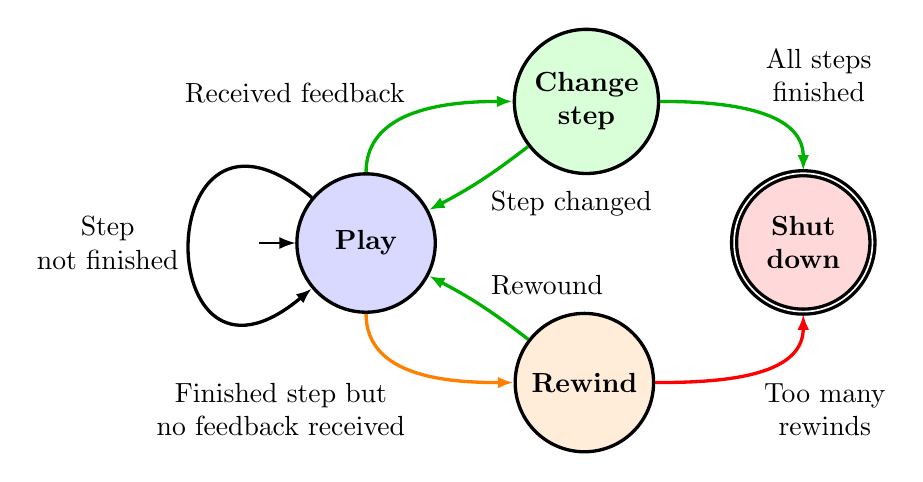
\begin{tikzpicture}[align=center,
    node distance=.5cm and 1.5cm,
    every initial by arrow/.style={-{Latex[length=2mm]}}]
    % Place nodes              
    \node [initial, very thick, state, minimum size=5em, initial text=, fill=white!85!blue] (play) {\textbf{Play}};
    \node [state, very thick, above right=of play, minimum size=5em, fill=white!85!green] (change) {\textbf{Change}\\\textbf{step}};
    \node [state, very thick, below right=of play, minimum size=5em, fill=white!85!orange] (rewind) {\textbf{Rewind}};
    \node [state, very thick, accepting, above right=of rewind, minimum size=5em, fill=white!85!red] (shutdown) {\textbf{Shut}\\\textbf{down}};

    % Draw edges
    \path[draw, -{Latex[length=2mm]}, very thick]
    (play) edge [out=270, in=180, color=red!50!yellow] node[below left, color=black] {Finished step but\\no feedback received} (rewind)
    edge [out=90, in=180, color=black!30!green] node[above left, color=black] {Received feedback} (change)
    edge [out=140, in=220,looseness=6] node[left] {Step\\not finished} (play)

    (change) edge [bend left=5, color=black!30!green] node[below right, color=black] {Step changed} (play)
    edge [out=0, in=90, color=black!30!green] node[above right, color=black] {All steps\\finished} (shutdown)

    (rewind) edge [bend right=5, color=black!30!green] node[above right, color=black] {Rewound} (play)
    edge [out=0, in=270, color=red] node[below right, color=black] {Too many\\rewinds} (shutdown);

\end{tikzpicture}\\
        \vspace{.1\textheight}%
        \onslide<2->{Currently working on a more thorough characterization of human behavior.}
    \end{center}
\end{frame}

\subsection{Implementation}
\begin{frame}{Implementation}
    \begin{center}
        \begin{tikzpicture}[align=center,
    arrow/.style={draw, thick, -{Latex[length=2mm]}},
    arrowr/.style={draw, thick, {Latex[length=2mm]}-}]

    % layers
    \pgfdeclarelayer{background0}
    \pgfdeclarelayer{background1}
    \pgfdeclarelayer{foreground}
    \pgfsetlayers{background0,background1,foreground}
    
    \begin{pgfonlayer}{foreground}
        \matrix[column sep=40mm, row sep=2mm, inner sep=2mm,
        every node/.style={text width=4em, text centered, minimum width=5em}] (mtx) {
            \node[draw, dashed, rectangle, anchor=center, inner sep=2mm, ] (usermodel) {User Model};
            & \node[draw, dashed, rectangle, anchor=center, inner sep=2mm] (app_backend) {App Backend};\\

            \node[inner sep=0mm] {}; %spacer
            & \node[anchor=center, inner sep=0mm] (docker) {Container};\\

            % spacers
            \node[inner sep=0mm, minimum height=1.5em] {};
            & \node[inner sep=0mm, minimum height=1.5em] {}; \\

            \node[anchor=center, inner sep=2mm, minimum height=5em] (emulator) {Client Emulator};
            & \node[anchor=center, inner sep=2mm, minimum height=5em] (control) {Control Backend};\\

            % spacers
            \node[inner sep=0mm, minimum height=.5em] {};
            & \node[inner sep=0mm, minimum height=.5em] {}; \\

            \node[inner sep=0mm, minimum height=2em] (label1) {Android Device}; 
            & \node[inner sep=0mm, minimum height=2em] (label2) {Cloudlet}; \\
        };

        \node[rectangle, draw, inner sep=2mm, right=15mm of control.25, 
        minimum width=20mm, minimum height=2em, fill=white!80!violet] (config) {Config};
        \node[rectangle, draw, inner sep=2mm, right=15mm of control.335, 
        minimum width=20mm, minimum height=2em, fill=white!80!violet] (trace) {Trace};
    \end{pgfonlayer}

    \begin{pgfonlayer}{background1}
        \node[fit=(usermodel) (emulator), draw, fill=white!80!yellow] (fit1) {};
        %\node[fit=(app_backend) (control)] (fit2) {};
        \node[fit=(docker) (app_backend), draw, fill=white!80!blue] (fit3) {};
        \node[fit=(control), draw, fill=white!80!red] (fit_control) {}; % just to make the size match
    \end{pgfonlayer}

    % main background fits
    \begin{pgfonlayer}{background0}
        \node[fit=(label1) (fit1), draw, fill=white!80!green] {};
        \node[fit=(label2) (fit_control) (fit3), draw, fill=white!80!black] {};
    \end{pgfonlayer}

    \begin{pgfonlayer}{foreground}
        % arrows
        % config and trace
        \draw[arrow] (config.west) -- (config.west -| fit_control.east);
        \draw[arrow] (trace.west) -- (trace.west -| fit_control.east);

        % between app and control backend
        \draw[arrowr] (fit_control.95) -- (fit_control.95 |- fit3.south);
        \draw[arrow] (fit_control.85) -- (fit_control.85 |- fit3.south);

        % between app and user model
        \draw[arrow] (app_backend.171) -- node[above] {Feedback Loop} (app_backend.171 -| fit1.east);
        \draw[arrowr] (app_backend.189) -- (app_backend.189 -| fit1.east);

        % between control and client
        \draw[arrow, dashed] (fit_control.155) -- node[above] {Config, Trace} (fit_control.155 -| fit1.east);
        \draw[arrowr, dashed] (fit_control.205) -- node[below] {Results} (fit_control.205 -| fit1.east);
    \end{pgfonlayer}

\end{tikzpicture}
    \end{center}
\end{frame}

\begin{frame}{Timestamping}
    \begin{center}
        \begin{sequencediagram}
    \newinst{client}{Client}
    \newinst[2]{cloudlet}{Cloudlet}

    \mess[1]{client}{Input $n$}{cloudlet}
    \node[inner sep=0, left=.15em of mess from] (t0) {$T_{s}$};
    \node[inner sep=0, right=.15em of mess to] (t1) {$T'_r$};


    \postlevel%
    \postlevel%
    \mess[1]{cloudlet}{Reply $n$}{client}
    \node[inner sep=0, right=.15em of mess from] (t3) {$T'_{s}$};
    \node[inner sep=0, left=.15em of mess to] (t4) {$T_r$};

\end{sequencediagram}
    \end{center}
\end{frame}

\subsection{Evaluation}
\begin{frame}{Evaluation}

\end{frame}

\section{Conclusions}
\begin{frame}{Conclusions}
    
\end{frame}

\end{document}